\documentclass{article}
\usepackage{ifthen,graphicx}
\usepackage[top=0.6in, bottom=0.9in, left=0.8in, right=0.8in]{geometry}
%\usepackage[top=1.0in, bottom=1.0in]{geometry}

%\pagestyle{empty}
\newboolean{KEY}
%\setboolean{KEY}{true}   %prints questions and answers
\setboolean{KEY}{false} %prints questions only
\newcommand{\answer}[1]{\ifthenelse{\boolean{KEY}}{#1}{}}
\newcommand{\titleheader}[2]{\ifthenelse{\boolean{KEY}}{#1}{#2}}

\begin{document}
\titleheader{\section*{CS170 SP2019 Final Exam Solution}}{\section*{CS170 SP2019 Final Exam}}

This is a close book, close note exam. Total points are 100. You have 50 minutes. \\

Name: \\

\begin{enumerate}
\item Briefly answer the following questions: [10]
  \begin{enumerate}
  \item What is a shell? What is a shell script.
  \vspace{1.0in}
  \answer{\emph{Shell is a command interpreter which will take user's command and communicate with the kernel to execute. Shell script is a simple program for shell to run.}}
  
  \item What is vim? What are the two major modes of vim?
  \vspace{1.0in}
  \answer{\emph{Command mode and input mode.}}
	
	\item What is Git? What is its difference with GitHub?
	\vspace{1.0in}
	
%	\item What does pull request do in Git?
%	\vspace{0.5in}	
	
	\item What are three stages in the compilation?
	\vspace{1.0in}
	
	\item How does the makefiles and make improve compilation?
	\vspace{1.0in}

  \end{enumerate}

\vspace{0.1in}

\item The shell script can work with command-line arguments. Explain the following symbols appear in the shell script. [5]
\begin{enumerate}
\item $\$0$
\item $\$1$
\item $\$2$
\item $\$*$
\item $\$\#$
\end{enumerate}

\answer{
\begin{enumerate}
\item $\$0$: name of the calling program (script)
\item $\$1$: the 1st positional argument exclude the name of the script
\item $\$2$: the 2nd positional argument exclude the name of the script
\item $\$*$: all the positional arguments
\item $\$\#$: number of positional arguments
\end{enumerate}
}

\newpage

\item Briefly explain the two commands in each pair: [12]
  \begin{enumerate}
  \item \texttt{pwd}  VS \texttt{ps} 
  \vspace{0.5in}
  \answer{\emph{pwd: current working directory; ps: display current running process}}
  
  \item \texttt{mkdir} VS \texttt{rmdir} 
  \vspace{0.5in}
  \answer{\emph{mkdir: create a directory; rmdir: delete a directory}}
  
  \item \texttt{less} VS \texttt{more}
  \vspace{0.5in}
  \answer{\emph{less: display the content of a file page-wise; more: display all the content of a file}}
  
  \item \texttt{head} VS \texttt{tail} 
  \vspace{0.5in}
  \answer{\emph{head: display top 10 lines of the file; tail: display last 10 lines of the file}}
	
	\item \texttt{cd ..} VS \texttt{cd .}
  \vspace{0.5in}
	\answer{\emph{go back to parent directory; stay in the current directory}}
	
	\item \texttt{mv} VS \texttt{cp}
\vspace{0.5in}
  \end{enumerate}
\vspace{0.5in}

%\item What Unix command could be used to solve the following question? [5]  
%\begin{enumerate}
%\item Search for a pattern in a file.
%\vspace{0.2in}
%\item Change the permission on a file or a directory.  
%\vspace{0.2in}
%\item Display information on disk usage by directory hierarchy and file.
%\vspace{0.2in}
%\item Displays the differences between two text files.
%\vspace{0.2in}  
%\item Display status information about processes running on the local system.
%\vspace{0.2in}
%\end{enumerate}

%\answer{\begin{enumerate}
%\item \emph{\texttt{grep}}
%
%\item \emph{\texttt{chmod}}
%
%\item \emph{\texttt{du}}
%
%\item \emph{\texttt{diff}}
%
%\item \emph{\texttt{ps}}
%
%\end{enumerate}}


\vspace{0.2in}
\item What do the following commands do? [22]
\begin{enumerate}
\item \texttt{chmod u+x file1.txt}
\vspace{0.5in}
\item \texttt{chmod go-w file2.txt} 
\vspace{0.5in}
%\item \texttt{sort -u file3.txt} 
%\vspace{0.5in}
%\item \texttt{wc -w file4.txt}
\item \texttt{./program1}
\vspace{0.5in}
\item \texttt{cat part2 part3 $>>$ book}
\vspace{0.5in}
\item \texttt{who $>$ whoson}
\vspace{0.5in}
\item \texttt{command1 $<$ someFile} 
\vspace{0.5in}
\item \texttt{cat file1 $|$ sort $|$ less}
\vspace{0.5in}  
\item \texttt{ps $|$ grep bash}
\vspace{0.5in}
\item \texttt{ls -l $|$ lpr}
\vspace{0.5in}
\item \texttt{kill 7324}
\vspace{0.5in}
\item \texttt{echo $\$\$$}
\vspace{0.5in}
\end{enumerate}


\answer{\begin{enumerate}
\item \emph{give user or owner execute permission on file1.txt}

\item \emph{remove write permission on file2.txt from group and everyone else}

\item \emph{display file3.txt without any duplicated lines}

\item \emph{count the total number of words in file4.txt}

\item \emph{A book file has been appended the content of two files: part2 and part3}

\item \emph{Write online user list to whoson file}

\item \emph{Using someFile as the input for command1}

\item \emph{Show sorted the file1 page-wise}

\item \emph{Search bash in the current process list}

\item \emph{Stop a process with ID 7324}

\item \emph{Display the PID of the current process}
\end{enumerate}}

\vspace{0.3in}
\item File system in Unix. Suppose the current working directory is \texttt{sue}. What are the absolute path and relative path for the \texttt{gcc} and \texttt{asg01.c} in the following diagram? [6] 
\begin{center}
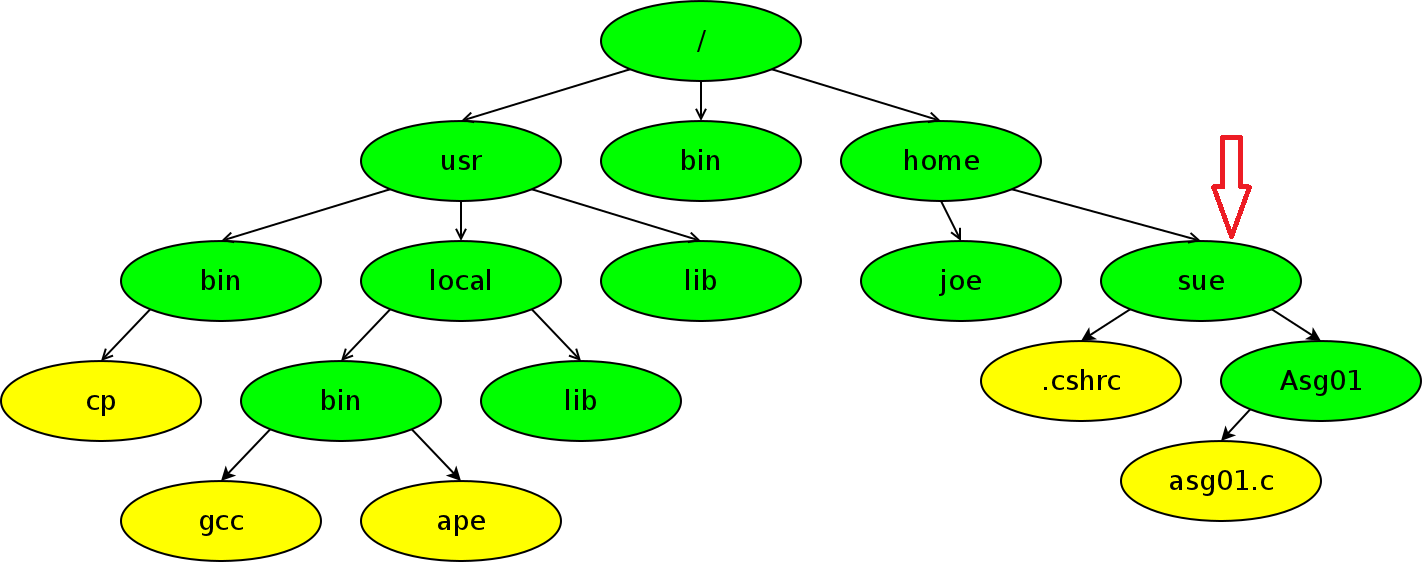
\includegraphics[width=0.55\textwidth]{unix_filesystem}
\end{center}
\vspace{1in}


\answer{\begin{enumerate}

\item \emph{absolute path starts with $/$: $/$home$/$mike$/$notes$/$textfile, relative path is notes$/$textfile}

\item \emph{absolute path starts with $/$: $/$home$/$gina$/$textfile, relative path is: ..$/$gina$/$textfile}

\end{enumerate}}

\vspace{0.8in}
%\item Circle the only one correct answer for the following questions related to the Git command [8]:
%\begin{enumerate}
%	\item Which command is used for changing the working directory to a new branch?
%	
%	\begin{tabular}{l l l l}
%	A. git push  & B. git pull & C. git fetch & D. git checkout \\
%	\end{tabular}
%	\vspace{0.1in}
%	\item Which command is used to copy the local change to the remote repository?
%	
%	\begin{tabular}{l l l l}
%	A. git push  & B. git pull & C. git fetch & D. git checkout \\
%	\end{tabular}
%	\vspace{0.1in}
%	\item Which command is used to copy the remote change to the local repository?
%	
%  \begin{tabular}{l l l l}
%	A. git push  & B. git pull & C. git merge & D. git checkout \\
%	\end{tabular}
%	\vspace{0.1in}
%  \item Which command is used to combine one branch into another?
%	
%  \begin{tabular}{l l l l}
%	A. git push  & B. git pull & C. git merge & D. git commit \\
%	\end{tabular}
%	\vspace{0.1in}
%		
%\end{enumerate}

\newpage
%\item Assuming the following files are in the working directory: 
%
%\begin{tabular}{l l l l l l}
%$\$ \texttt{ls}$ & & & & &\\
%intro & notesb & ref2 & section1 & section3 & section4b \\
%notesa & ref1  & ref3 & section2 & section4a & sentrev \\
%\end{tabular}
%
%What are the results after executing the following commands? [9]
%\begin{enumerate}
%\item \texttt{ls sec*}
%\vspace{0.5in}
%\item \texttt{ls ref?} 
%\vspace{0.5in}
%\item \texttt{ls section[1-3]}  
%\vspace{0.5in}
%\item \texttt{ls i*}
%\vspace{0.5in}
%\item \texttt{ls *[13]} 
%\vspace{0.5in}
%\item \texttt{ls note?[ab]} 
%\vspace{0.5in}
%\end{enumerate}
%
%\answer{\begin{enumerate}
%\item \emph{section1 section3 section4b section2 section4a}
%
%\item \emph{ref2 ref1 ref3}
%
%\item \emph{section1 section2 section3}
%
%\item \emph{intro}
%
%\item \emph{section1 ref1 ref3}
%
%\item \emph{notesa notesb}
%
%\end{enumerate}}
%
%\vspace{0.3in}


\item Shell script coding problems:[45]
\begin{enumerate} 
\item Write a script that displays (sends to standard output) the name
of the calling program, the number of positional parameters, and a list of
positional parameters. [6]
\vspace{3in}



\item Write a shell  that prompt the user with "$>>$" and read a string of text
from the user. If the user enters a nonnull string, the scirpt displays "You entered: " followed by the string; 
otherwise it displays "Where is your input?". [6]

\vspace{2in}

\newpage
\item Write a short script that tells you whether the permissions for two files, whose
names are given as arguments to the script, are identical. If the permissions for
the two files are identical, output the common permission field. Otherwise, output
each filename followed by its permission field. [12]\\
(Hint: Using ls -l to display permission and cut utility.) \\
\texttt{$\$$ ls -l dog} \\
\texttt{-rw-r--r-- 1 max max 0 2012-10-15 12:20 dog}\\
\vspace{4in}

\item Write a shell script that prompt the user for a file name then check if this file exists 
in the current directory. If file exists, copies the file named to a file with the same name 
with the filename extension of \textbf{.bak}. Otherwise a file is created in the current directory 
and a corresponding message is displayed. [8]

\answer{
\texttt{$\#$!$\/$bin$\/$bash}
\texttt{read -p "`Enter a string:"' ufile}
}

\newpage
%\item Write a short script that prompt the user for an age, then use \textbf{case} to check
%the value of age if the age is between 0 to 4, echo a message saying too young to go to school;
%if the age is 5, echo a message saying go to kindergarten; if the age is between 6 to 17, echo a
%message saying go to the corresponding grade (eg. 6 will go to the 1 grade so on and so forth).
%Default will echo a message saying too old for school. [13]
\item Write a shell script that can provide following \textbf{a, b, c, d} menus for the user. If user enter other than \textbf{a, b, c, d}, the program exit. [13]
\begin{itemize}
\item \textbf{a.} Display user currently logged in 
\item \textbf{b.} List current running processes 
\item \textbf{c.} List only the permission of all the files and directories under current directory
\item \textbf{d.} Go back to its parent's directory
\end{itemize}

\end{enumerate} 

\end{enumerate}
\end{document}